\chapter{Validación}
\thispagestyle{empty}

\section{Análisis} \label{sec:\thesection}
En este capítulo se mostrarán los ensayos realizados para validar los requerimientos presentados en la sección \ref{sec:1.5}. Esto incluye:
\begin{itemize}
	\item \textbf{REQ-01:} validar que firmware desarrollado para el equipo maneja correctamente todas las entradas y salidas.
	\item \textbf{REQ-02:} validar que la carga sigue la posición y velocidad indicada por DMX .
	\item \textbf{REQ-03:} validar que el comportamiento del sistema ante el descubrimiento de uno de los 3 errores detectables es la esperada. 
	\item \textbf{REQ-04:} verificar que el funcionamiento del dipswitch es correcto.
\end{itemize}

\section{Validación del requerimiento REQ-03} \label{sec:\thesection}
Para validar el requerimiento REQ-03 se realizaron 3 pruebas.
\subsection{Pérdida de DMX}
Si el equipo recibe señal de DMX el led externo debe cambiar de estado a razón de 4 veces por segundo, y mantener el estado si se perdió la señal por más de un segundo.

Para verificar que esto se realizaron las siguientes pruebas:
\begin{enumerate}
	\item Se conectó el equipo a la red, sin el cable de DMX conectado. El led externo se mantiene apagado.
	\item Se conecto el cable DMX con la consola prendida. El led externo comienza a parpadear a una frecuencia de 2Hz.
	\item Se desconecta el cable DMX de la consola. El led externo deja de parpadear transcurrido 1 segundo de haber desconectado el cable.
\end{enumerate}
Con esto se verifica que el comportamiento es el deseado.	
	 
\subsection{Accionamiento indebido del fin de carrera}
Idealmente, el fin de carrera solo debe accionarse una vez durante la rutina de calibración para determinar el 0 de posición. En caso de que se accione fuera de este escenario la carga debe frenar por 6 segundos, y volver a subir al 0 de posición. En caso que el FDC esté presionado por más de 15 segundos se debe parar el motor, poner el freno, y el led interno debe cambiar de estado cada 2 segundos.

Para verificar que esto se realizaron las siguientes pruebas:
\begin{enumerate}
	\item Luego de que la etapa de calibración concluye, se le indica al equipo que baje la carga 2 metros (velocidad al 50\%). Durante el descenso se acciona el fin de carrera una vez y se espera. Al accionarlo, la carga para durante 6 segundos, y comienza a subir lentamente al 0 de posición. Luego intenta bajar nuevamente y llega a la posición deseada.
	\item Partiendo de una posición de 2 metros, se le indica al equipo que suba la carga 1 metro (velocidad al 50\%). Durante el ascenso se acciona el fin de carrera una vez y se espera. Al accionarlo, la carga para durante 6 segundos, y comienza a subir lentamente al 0 de posición. Luego intenta subir nuevamente y llega a la posición deseada.
	\item Partiendo de una posición de 1 metro, se mantiene presionado el fin de carrera. Durante este tiempo la carga baja lenta y continuamente hasta que pasan 15 segundos. En ese momento la carga para, se activa el freno, y el led interno titila a una frecuencia de 0.25Hz.
\end{enumerate}

El comportamiento en la tercer prueba es el esperado ya que como se mantiene el fin de carrera presionado automáticamente "se llega al 0", y en consiguiente la carga baja 10 cm, como es de esperarse. Luego se pasa al modo normal, pero como el fin de carrera sigue presionado se vuelve a entrar al de calibración, y el ciclo vuelve a comenzar denuevo, repitiendose hasta que transcurren 15 segundos.

Por lo tanto, con esto se verifica que el comportamiento es el deseado.
	
\subsection{Corte de cadena}
Si la relación entre el encoder de disco y de motor se desvía mucho de la dada por la tabla \ref{table:3.2} el se debe detener el motor y accionar el freno para evitar que la carga baje. Además, el led interno debe cambiar de estado 2 veces por segundo.

Para verificar que esto se realizaron las siguientes pruebas:
\begin{enumerate}
	\item Se desconecta el cable que asocia el encoder del motor y la placa de controlcausando que las cuentas del encoder de motor dejen de cambiar. Luego de un segundo el motor para y el freno se acciona, deteniendo completamente la carga. Adicionalmente, el led interno titila a una frecuencia de 1Hz.
	\item Se desconecta el cable que asocia el encoder del disco y la placa de control  causando que las cuentas del encoder de disco dejen de cambiar. Luego de un segundo el motor para y el freno se acciona, deteniendo completamente la carga. Adicionalmente, el led interno titila a una frecuencia de 1Hz.
\end{enumerate}
Para verificar completamente que el comportamiento ante un error es el deseado se debería, además de probar la pérdida de cuenta de los encoders, probar cortando la cadena. Como no se logró hacer esto con el equipo en funcionamiento este punto no se pudo validar totalmente. Sin embargo, es muy poco probable que se corte la cadena debido a la dureza de la misma y a que la carga es de solamente 3 Kg.

\section{Validación de los requerimientos REQ-01, 02 y 04} \label{sec:\thesection}
Los requerimientos REQ-01, REQ-02 y REQ-04 se validan simplemente controlando al updown mediante DMX. De esta manera se verifica funcionamiento de todos ellos ya que se utilizan todas las entradas y salidas (asociado a la validación del REQ-01), el sistema de control (asociado a la validación del REQ-02) y el dipswitch (asociado a la validación del REQ-04).

La prueba se realiza con 4 equipos updown dispuestos en forma de matriz de 2x2, como se muestra en la figura \ref{fig:4.1}, colgados a 4 metros sobre el nivel del piso. Todos tienen en su extremo una carga de 3Kg, que es una luminaria cuyas intensidades R, G y B pueden ser controladas mediante 3 canales de DMX.

\begin{figure}[!ht]
	\centering
	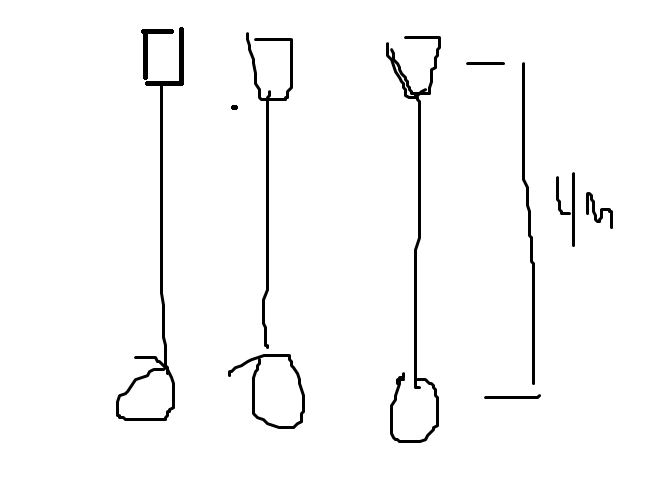
\includegraphics[width=15cm,scale=1]{resources/4_1-disposicionUpdowns.png}
	\caption{Disposición de los equipos Updown}
	\label{fig:\thefigure}
\end{figure}

Para manejar los equipos se utiliza la consola \href{http://www.lighttrader.com/images/HI61020007_L.JPG}{HedgeHog 4}, de HighEnd Systems. En ella se programan 2 rutinas:
\begin{itemize}
	\item \textbf{Rutina 1}: los 4 equipos se mueven juntos, a velocidad máxima, a las posiciones 0, 1, 2, 3 y 4 metros, en subida y en bajada.
	\item \textbf{Rutina 2}: los 4 equipos se mueven a posiciones distintas (apelando al direccionamiento por dip switch) y la velocidad varía con el tiempo.
\end{itemize}

\subsection{Direccionamiento de los equipos}
Cada updown recibe 2 canales DMX, uno de posición y otro de velocidad, mientras que las cargas, que se configuran independientemente, reciben 3 canales (R, G y B). Además, en las instalaciones de equipos DMX por convención los equipos se direccionan de atras para adelante, de izquierda a derecha.

Esto quiere decir que, referido a la figura \ref{fig:4.1}, el updown A tendrá la dirección 1, el B la dirección 3, el C la 5 y el D la 7. Para lograr esto se configuran los dipswitch como corresponde. Por ejemplo, el dipswitch del equipo C tendrá la llave 2 y 3 activadas, lo cual se traduce a address 5 en el programa.\\
Por otro lado, las cargas se las configura en la dirección 10. Esto se hace manualmente desde un display digital que las luminarias traen. 

En la figura \ref{fig:4.2} se muestra cómo se vizualizan los canales en la consola HOG, y a qué estará asociado cada uno. 

\begin{figure}[!ht]
	\centering
	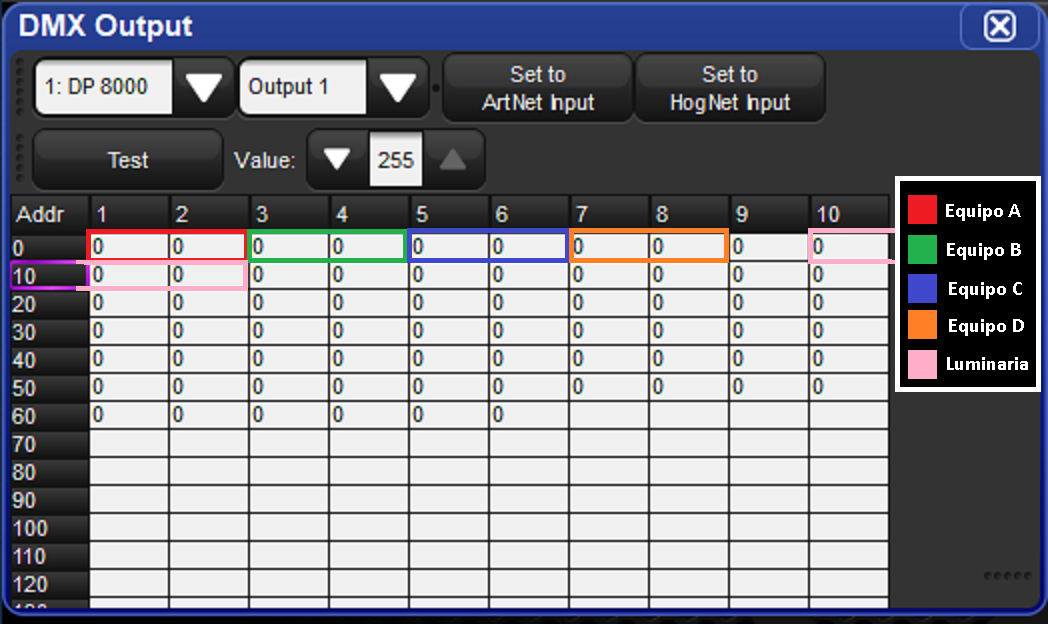
\includegraphics[width=15cm,scale=1]{resources/4_2-direccionamiento.png}
	\caption{Canales DMX asociados a los updown y las cargas}
	\label{fig:\thefigure}
\end{figure}

\subsection{Rutina 1}
Se programa en la consola la \textit{cuelist} (secuencia de entradas) mostrada en la figura \ref{fig:4.3}. Como se ve en la figura el patrón que siguen todas las car
	
\begin{figure}[!ht]
	\centering
	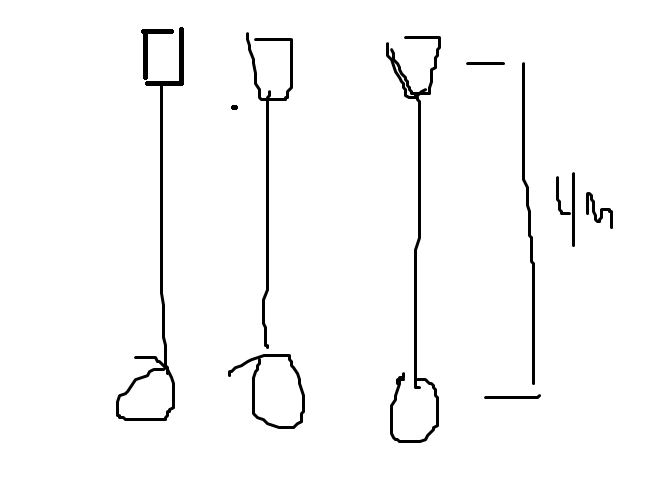
\includegraphics[width=15cm,scale=1]{resources/4_3-cuelist1.png}
	\caption{Cuelist 1}
	\label{fig:\thefigure}
\end{figure}

\subsection{Rutina 2}







